



\chapter{Vecteurs et translations}


\section{Notion de vecteurs}
\subsection{Translation de vecteur $\overrightarrow{AB}$}

\begin{minipage}[c]{0.6\linewidth}
Sur la figure ci-contre, on a construit l'image $(F_2)$ de la figure $(F_1)$ par la translation qui transforme $A$ en $B$. \\
La flèche que l'on a tracée allant de $A$ jusqu'à $B$ indique la direction, le sens et la longueur du déplacement que l'on doit effectuer pour construire l'image d'un point. 
\end{minipage} \hfill
\begin{minipage}[c]{0.3\linewidth}
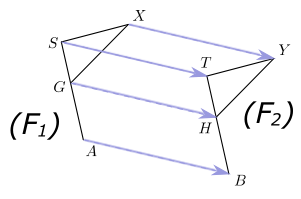
\includegraphics[scale=.7]{drapeau}
\end{minipage}


\begin{Définition}
Soit $A$ et $B$ deux points distincts du plan. \\
La translation qui transforme $A$ en $B$ est appelée {\bf{translation de vecteur $\overrightarrow{AB}$}}.

\end{Définition}

\vspace{0.5cm}

\begin{Propriété}$ $\\
\vspace{-0.5cm}
\begin{minipage}[c]{0.7\linewidth}
Lorsque $A$ et $B$ sont distincts, le vecteur $\overrightarrow{AB}$ est caractérisé par : 
\begin{itemize}[label=\textcolor{Couleur2}{$\bullet$}]
\item sa {\bf{direction}} : celle de la droite $(AB)$ ;
\item son {\bf{sens}} : de $A$ vers $B$ ; 
\item sa {\bf{longueur}} : la longueur $AB$.
\end{itemize}

Cette longueur est appelée {\bf{norme}} du vecteur $\overrightarrow{AB}$. On la note $\left\Vert\overrightarrow{AB}\right\Vert$.

\end{minipage} \hfill
\begin{minipage}[c]{0.2\linewidth}
\begin{tikzpicture}
\draw[->,>=latex,Couleur8] (0,0) node {$.$} -- (2,0) node {$.$};
\draw (0,0) node[above] {$A$};
\draw (2,0) node[above] {$B$};
\draw (1,0) node[below] {$\overrightarrow{AB}$};
\end{tikzpicture}
\end{minipage}


\end{Propriété}

\vspace{0.5cm}

\begin{Méthode}Construire l'image d'une figure par une translation\\
Construire l'image $M'N'O'P'$ du trapèze $MNOP$ la translation de vecteur $\overrightarrow{AA'}$.

\begin{center}
\begin{tikzpicture}[x=0.6cm,y=0.6cm]
% Définition des limites
\def\xmin{-6}
\def\xmax{8}
\def\ymin{-4}
\def\ymax{4}

% Grille 1x1 pour chaque carreau (avec step=1 pour correspondre aux coordonnées)
\draw[Couleur3!30] (\xmin,\ymin) grid [step=1] (\xmax,\ymax);

% Vecteur de translation
\draw[->,>=latex,Couleur8,thick] (-5,3) -- (-1,4);
\draw (-5,3) node[below] {$A$};
\draw (-1,4) node[below] {$A'$};

% Polygone BCDEB
\draw[thick] (-3,2) node[left] {$M$} -- (0,-2) node[below left] {$P$} -- (3,-3) node[below left] {$O$} -- (3,0) node[below left] {$N$} -- (-3,2);

\end{tikzpicture}
\end{center}

\end{Méthode}

\newpage

\subsection{Égalité de deux vecteurs}
\begin{minipage}[c]{0.7\linewidth}
\begin{Définition}
Soit $A$, $B$, $C$ et $D$ quatre points.\\
Les vecteurs $\overrightarrow
{AB}$ et $\overrightarrow{CD}$ sont égaux signifie que $D$ est l'image de $C$ par la translation de vecteurs $\overrightarrow{AB}$. \\On note $\overrightarrow{AB}=\overrightarrow{CD}$.

\end{Définition}

\begin{Propriété}
Soit $A$, $B$, $C$ et $D$ quatre points.
\begin{enumerate}
\item Les vecteurs $\overrightarrow{AB}$ et $\overrightarrow{CD}$ sont égaux si, et seulement si, ils ont même direction, même sens et même norme.
\item $\overrightarrow{AB}=\overrightarrow{CD}$ si, et seulement si, les segments $[AD]$ et $[BC]$ ont le même milieu.
\item $\overrightarrow{AB}=\overrightarrow{CD}$ si, et seulement si, $ABDC$ est un parallélogramme.
\end{enumerate}

\end{Propriété}
\end{minipage} \hfill
\begin{minipage}[c]{0.3\linewidth}
\begin{center}
\begin{tikzpicture}
 [x=0.7cm,y=0.7cm]


\draw[->,>=latex,Couleur8] (-5,3) node[above] {$\color{black}{A}$} -- (-1,4) node[above] {$\color{black}{B}$};
\draw[cyan] (-5,3)--(-3,1);
\draw[cyan] (-1,4)--(1,2);
\draw[YellowGreen] (-5,3)--(1,2);
\draw[YellowGreen] (-1,4)--(-3,1);
\draw[->,>=latex,Couleur8] (-3,1) node[below] {$\color{black}{C}$} -- (1,2) node[below] {$\color{black}{D}$};
\draw (-3.5,2.75) node{$\|$} ;  
\draw (-0.5,2.25) node{$\|$} ;  
\draw (-1.5,3.25) node{$\backslash$} ;  
\draw (-2.5,1.75) node{$\backslash$} ;  
\draw (-2,2.5) node[below]{$I$} ;  
\end{tikzpicture}
\end{center}
\end{minipage}






\begin{Remarque}
Dans la propriété $\color{Couleur6}{3.}$, $ABDC$ peut être un parallélogramme aplati.\\
D'après la propriété $\color{Couleur6}{2.}$, $\overrightarrow{AI}=\overrightarrow{IB}$ si, et seulement si, $[AB]$ et $[II]$ ont le même milieu. En convenant que le milieu de $[II]$ est le point $I$, on obtient la propriété suivante.

\end{Remarque}

\begin{Propriété} $ $\\
\vspace{-0.5cm}
\begin{minipage}[c]{0.6\linewidth}
Soit $A$ et $B$ deux points distincts.\\
Le point $I$ est le milieu de $[AB]$ si, et seulement si, $\overrightarrow{AI}=\overrightarrow{IB}$.
\end{minipage} \hfill
\begin{minipage}[c]{0.3\linewidth}
\begin{tikzpicture}
\draw[->,>=latex,Couleur8] (0,0) node[above] {$\color{black}{A}$} -- (1,0) node[above] {$\color{black}{I}$};
\draw[->,>=latex,Couleur6] (1,0)  -- (2,0) node[above] {$\color{black}{B}$};

\draw (0.5,0) node[below] {$\overrightarrow{AI}$};
\draw (1,-0.3) node[below] {$=$};
\draw (1.5,0) node[below] {$\overrightarrow{IB}$};
\end{tikzpicture}
\end{minipage}
\vspace{0.5cm}
\end{Propriété}


\subsection{Vecteur $\overrightarrow{u}$}


\begin{center}
\begin{tikzpicture}[x=0.4cm,y=0.4cm]
% Définition des limites
\def\xmin{-4}
\def\xmax{6}
\def\ymin{-5}
\def\ymax{4}

% Axes
\draw[->] (\xmin,0) -- (\xmax,0) node[right] {$x$};
\draw[->] (0,\ymin) -- (0,\ymax) node[above] {$y$};

% Grille avec step=1 pour correspondre aux coordonnées
\draw[Couleur6!30] (\xmin,\ymin) grid[step=1] (\xmax,\ymax);


% Vecteurs de translation
\draw[->,>=latex,Couleur8,thick] (-2,1) -- (1,3);
\draw (-2,1) node[above] {$A$};
\draw (1,3) node[above] {$B$};

\draw[->,>=latex,Couleur8,thick] (1,1) -- (4,3);
\draw (1,1) node[above] {$C$};
\draw (4,3) node[above] {$D$};

\draw[->,>=latex,Couleur8,thick] (-3,-2) -- (0,0);
\draw (-3,-2) node[above] {$E$};
\draw (0,0) node[above right] {$F$};

\draw[->,>=latex,Couleur8,thick] (-1,-3) -- (2,-1);
\draw (-1,-3) node[above] {$G$};
\draw (2,-1) node[above] {$H$};

% Vecteur de référence
\draw[->,>=latex,Couleur8,thick] (2,-4) -- (5,-2);
\draw (3.5,-3) node[below]{$\overrightarrow{u}$};

\end{tikzpicture}
\end{center}


\noindent Sur la figure ci-contre, la translation de vecteur $\overrightarrow{AB}$ transforme $C$ en $D$, $E$ en $F$ et $G$ en $H$. \\On a donc $\overrightarrow{AB}=\overrightarrow{CD}=\overrightarrow{EF}=\overrightarrow{GH}$.\\
$\overrightarrow{AB}$, $\overrightarrow{CD}$, $\overrightarrow{EF}$ et $\overrightarrow{GH}$ sont des {\bf{représentants}} d'un même vecteur, que l'on peut convenir d'appeler par une seule lettre, par Exemple $\overrightarrow{u}$. \\
Tous ces représentants ont la même direction, le même sens et la même norme.\\
$\overrightarrow{AB}$ est le représentant d'{\bf{origine}} $A$ du vecteur $\overrightarrow{u}$. Son {\bf{extrémité}} est le point $B$.


\begin{Remarque}
Un vecteur a une infinité de représentants.
\end{Remarque}



\begin{Définition}
Le vecteur dont les représentants sont $\overrightarrow{AA}$, $\overrightarrow{BB}$, $\overrightarrow{CC}$,$\ldots$ est appelé le {\bf{vecteur nul}}.\\
 On le note $\overrightarrow{0}$.

\end{Définition}

\section{Somme de deux vecteurs}

\begin{Définition} $ $\\
\vspace{-0.5cm}
\begin{minipage}[c]{0.68\linewidth}
La somme de deux vecteurs $\overrightarrow{u}$ et $\overrightarrow{v}$ est le vecteur associé à la translation résultant de l'enchaînement des translations de vecteur $\overrightarrow{u}$ et de vecteur $\overrightarrow{v}$. \\On note ce vecteur $\overrightarrow{u}+\overrightarrow{v}$ 
\end{minipage} \hfill
\begin{minipage}[c]{0.26\linewidth}
\begin{center}
\begin{tikzpicture}
 [x=0.7cm,y=0.7cm]
\draw[->,>=latex,Couleur6] (0,-1) node[above left] {$\color{black}{A}$} -- (2,0) node[above] {$\color{black}{B}$};
\draw[->,>=latex,Couleur8] (2,0)  -- (3,-2) node[below right] {$\color{black}{C}$};
\draw[->,>=latex,YellowGreen] (0,-1)  -- (3,-2);
\draw[Couleur6] (1,-0.5) node[above] {$\overrightarrow{u}$};
\draw[Couleur8] (2.5,-1) node[right] {$\overrightarrow{v}$};
\draw[YellowGreen] (1.5,-1.7) node[below] {$\overrightarrow{u}+\overrightarrow{v}$};
\end{tikzpicture}
\end{center}
\end{minipage}
\vspace{0.5cm}
\end{Définition}

\newpage

\begin{Théorème}
Pour tous les points $A$, $B$, $C$ et $D$ : 
\begin{itemize}[label=\textcolor{Couleur1}{$\bullet$}]
\item {\bf{Relation de Chasles : }} $\overrightarrow{AB}+\overrightarrow{BC}=\overrightarrow{AC}$
\item $\overrightarrow{AB}+\overrightarrow{AC}=\overrightarrow{AD}$ si, et seulement si, le quadrilatère $ABDC$ est un parallélogramme.
\end{itemize}

\end{Théorème}


\begin{minipage}[c]{0.45\linewidth}
{\color{Couleur6}{1.}}Si $\overrightarrow{AB}$ est un représentant de $\overrightarrow{u}$ et $\overrightarrow{BC}$ est un représentant de $\overrightarrow{v}$ on a : \\

\begin{center}
\begin{tikzpicture}
[x=0.7cm,y=0.7cm]
\draw[->,>=latex,Couleur6] (2,-1) node[above left] {$\color{black}{A}$} -- (4,0) node[above] {$\color{black}{B}$};
\draw[->,>=latex,Couleur8] (4,0)  -- (5,-2) node[below right] {$\color{black}{C}$};
\draw[->,>=latex,YellowGreen] (2,-1)  -- (5,-2);
\draw[Couleur6] (3,-0.5) node[above] {$\overrightarrow{u}$};
\draw[Couleur8] (4.5,-1) node[right] {$\overrightarrow{v}$};
\draw[YellowGreen] (3.5,-1.7) node[below] {$\overrightarrow{u}+\overrightarrow{v}$};
\draw[->,>=latex,Couleur6] (2,0.2)  -- (4,1.2) ;
\draw[->,>=latex,Couleur8] (5.2,0.5)  -- (6.2,-1.5) ;
\draw[Couleur6] (3,0.8) node[above] {$\overrightarrow{u}$};
\draw[Couleur8] (5.8,-0.4) node[right] {$\overrightarrow{v}$};
\end{tikzpicture}
\end{center}
\end{minipage}
 \hfill
\begin{minipage}[c]{0.45\linewidth}
{\color{Couleur6}{2.}}Si $\overrightarrow{AB}$ est un représentant de $\overrightarrow{u}$ et $\overrightarrow{AC}$ est un représentant de $\overrightarrow{v}$ on a : \\

\begin{center}
\begin{tikzpicture}
 [x=0.7cm,y=0.7cm]
\draw[<-,>=latex,Couleur6] (-1,-1) node[above left] {$\color{black}{B}$} -- (2,0) node[above] {$\color{black}{A}$};
\draw[->,>=latex,Couleur8] (2,0)  -- (2,-2) node[below right] {$\color{black}{C}$};
\draw[->,>=latex,YellowGreen] (2,0)  -- (-1,-3)node[below right] {$\color{black}{D}$};
\draw[dotted] (-1,-1)-- (-1,-3);
\draw[dotted] (2,-2)-- (-1,-3);
\draw[Couleur6] (0.2,-0.5) node[above] {$\overrightarrow{u}$};
\draw[Couleur8] (2,-1) node[right] {$\overrightarrow{v}$};
\draw[YellowGreen] (0.8,-1.8) node[below] {$\overrightarrow{u}+\overrightarrow{v}$};
\draw[<-,>=latex,Couleur6] (-0.5,0.2)  -- (2.5,1.2) ;
\draw[->,>=latex,Couleur8] (3.2,0.5)  -- (3.2,-1.5) ;
\draw[Couleur6] (1,0.8) node[above] {$\overrightarrow{u}$};
\draw[Couleur8] (3.2,-0.4) node[right] {$\overrightarrow{v}$};
\end{tikzpicture}
\end{center}
\end{minipage}


\begin{minipage}[c]{0.7\linewidth}
D'après la relation de Chasles, $\overrightarrow{AB}+\overrightarrow{BA}=\overrightarrow{AA}=\overrightarrow{0}$. \\On a donc $\overrightarrow{AB}+\overrightarrow{BA}=\overrightarrow{0}$. \\On dit que le vecteur $\overrightarrow{BA}$ est {\bf{l'opposé}} du vecteur $\overrightarrow{AB}$ et on note : $\overrightarrow{BA}=-\overrightarrow{AB}$.
\end{minipage} \hfill
\begin{minipage}[c]{0.25\linewidth}
\begin{tikzpicture}
\draw[->,>=latex,Couleur6] (0,0) node[above] {$\color{black}{A}$} -- (3,0) node[above] {$\color{black}{B}$};
\draw[<-,>=latex,Couleur8] (0,-1) node[above] {$\color{black}{A}$} -- (3,-1) node[above] {$\color{black}{B}$};

\draw[Couleur6] (1.5,0) node[below] {$\overrightarrow{AB}$};
\draw[Couleur8] (1.5,-1) node[below] {$\overrightarrow{BA}=-\overrightarrow{AB}$};
\end{tikzpicture}
\end{minipage}

\begin{Propriété}
Soit $\overrightarrow{u}$, $\overrightarrow{v}$ et $\overrightarrow{w}$ trois vecteurs.
\vspace{-0.5cm}
\begin{multicols}{2}
\begin{itemize}[label=\textcolor{Couleur2}{$\bullet$}]
\item $\overrightarrow{u}+\overrightarrow{v}=\overrightarrow{v}+\overrightarrow{u}$
\item $(\overrightarrow{u}+\overrightarrow{v})+\overrightarrow{w}=\overrightarrow{u}+(\overrightarrow{v}+\overrightarrow{w})=\overrightarrow{u}+\overrightarrow{v}+\overrightarrow{w}$
\item $\overrightarrow{u}+\overrightarrow{0}=\overrightarrow{u}$
\item $\overrightarrow{u}-\overrightarrow{v}=\overrightarrow{u}+(-\overrightarrow{v})$
\end{itemize}
\end{multicols}
\end{Propriété}



\section{Produit d'un vecteur par un réel}

\begin{Définition} $ $\\
\vspace{-0.5cm}
\begin{itemize}[label=\textcolor{Couleur6}{$\bullet$}]
\item Si $k$ est un nombre réel non nul et $\overrightarrow{u}\neq \overrightarrow{0}$.\\
$k\overrightarrow{u}$ est le vecteur défini par : \begin{enumerate}
\item sa direction : $k\overrightarrow{u}$ et $\overrightarrow{u}$ ont la même direction ; 
\item sons sens : si $k>0$, $k\overrightarrow{u}$ a le même sens que $\overrightarrow{u}$ ; si $k<0$, $k\overrightarrow{u}$ et $\overrightarrow{u}$ sont de sens contraires ; 
\item sa norme : $\left\Vert k\overrightarrow{u}\right\Vert =\vert k \vert \times \left\Vert \overrightarrow{u}\right\Vert $
\end{enumerate}
\item Si $k=0$, $0\overrightarrow{u}=\overrightarrow{0}$ et si $\overrightarrow{u}=\overrightarrow{0}$, $k\overrightarrow{0}=\overrightarrow{0}$.
\end{itemize}
\end{Définition}



\begin{Exemple}
\hspace{0.5cm}\begin{center}
 \begin{tikzpicture}[x=0.5cm,y=0.5cm]
% Définition des limites
\def\xmin{-6}
\def\xmax{6}
\def\ymin{-6}
\def\ymax{4}



% Grille
\draw[gray!30] (\xmin,\ymin) grid [step=1] (\xmax,\ymax);

% Vecteur de référence u
\draw[->,>=latex,Couleur8,thick] (2,-4) -- (5,-2);
\draw[Couleur8] (3.5,-3) node[below]{$\overrightarrow{u}$};

% Multiples du vecteur u
\draw[->,>=latex,Couleur6,thick] (0,2) -- (1.5,3);
\draw[Couleur6] (0,4) node[below]{};

\draw[->,>=latex,violet,thick] (5,2) -- (-4,-4);
\draw[violet] (0,0.2) node[below]{};

\draw[->,>=latex,Couleur3,thick] (-2,-4) -- (4,0);
\draw[Couleur3] (2,-1.7) node[below]{};

\draw[->,>=latex,Couleur11,thick] (2,2) -- (-4,-2);
\draw[Couleur11] (-1.5,1.5) node[below]{};

\end{tikzpicture}
\end{center}

\end{Exemple}


\begin{Remarque}
Les droites portées par les vecteurs $\overrightarrow{u}$ et $k\overrightarrow{u}$ sont parallèles.
\end{Remarque}



\begin{Propriété}
Soit $\overrightarrow{u}$, $\overrightarrow{v}$ deux vecteurs, et $k$, $k'$ deux réels.
\vspace{-0.5cm}
\begin{multicols}{3}
\begin{itemize}[label=\textcolor{Couleur2}{$\bullet$}]
\item $k(\overrightarrow{u}+\overrightarrow{v})=k\overrightarrow{u}+k\overrightarrow{v}$
\item $(k+k')\overrightarrow{u}=k\overrightarrow{u}+k'\overrightarrow{u}$
\item $k(k'\overrightarrow{u})=(kk')\overrightarrow{u}$
\end{itemize}
\end{multicols}
\end{Propriété}

\begin{Exemple}
Soit $\overrightarrow{u}$, $\overrightarrow{v}$ deux vecteurs.
\vspace{-0.5cm}
\begin{multicols}{3}
\begin{itemize}[label=\textcolor{Couleur8}{$\bullet$}]
\item $2(\overrightarrow{u}+\overrightarrow{v})=$ \ligne
\item $2\overrightarrow{u}+3\overrightarrow{u}=$ \ligne
\item $4(5\overrightarrow{u})=$ \ligne
\end{itemize}
\end{multicols}
\end{Exemple}



\begin{Propriété} $ $\\
\vspace{-0.5cm}
\begin{minipage}[c]{0.6\linewidth}
$I$ est le milieu du segment $[AB]$ si, et seulement si, $\overrightarrow{AI}=\dfrac{1}{2}\overrightarrow{AB}$
\end{minipage} \hfill
\begin{minipage}[c]{0.3\linewidth}
\begin{tikzpicture}
\draw[->,>=latex,Couleur8] (0,-0.05)  -- (1,-0.05) node[above] {$\color{black}{I}$};
\draw[->,>=latex,Couleur6] (0,0) node[above] {$\color{black}{A}$} -- (2,0) node[above] {$\color{black}{B}$};

\draw[Couleur8] (1,0) node[below] {$\overrightarrow{AI}{\color{black}{=\dfrac{1}{2}}}{\color{Couleur6}{\overrightarrow{AB}}}$};
\end{tikzpicture}
\end{minipage}
\vspace{0.5cm}
\end{Propriété}

\bigskip

\newpage

\section*{Exercices - Vecteurs et translations}
\addcontentsline{toc}{section}{Exercices}
{\setlength{\columnseprule}{0pt}
\setcounter{NumEx}{1}

\subsection*{Notion de vecteur}


%https://www.mathoutils.fr/wp-content/uploads/2022/08/03-Exercices.pdf

\begin{minipage}{0.6\textwidth}

\begin{Exercice} %1
Déterminer les vecteurs égaux aux vecteurs $\overrightarrow{u}$ et $\overrightarrow{v}$.

\end{Exercice}

\begin{Exercice} %2
Construire les points L et M tels que $ \overrightarrow{GL}=\overrightarrow{u} $ et
$ \overrightarrow{KM}=\overrightarrow{v} $.

\end{Exercice}

\begin{Exercice} %3
Construire le point N tel que $ \overrightarrow{JN}=\overrightarrow{EH} $.

\end{Exercice}
\end{minipage}
\begin{minipage}{0.35\textwidth}
\begin{center}
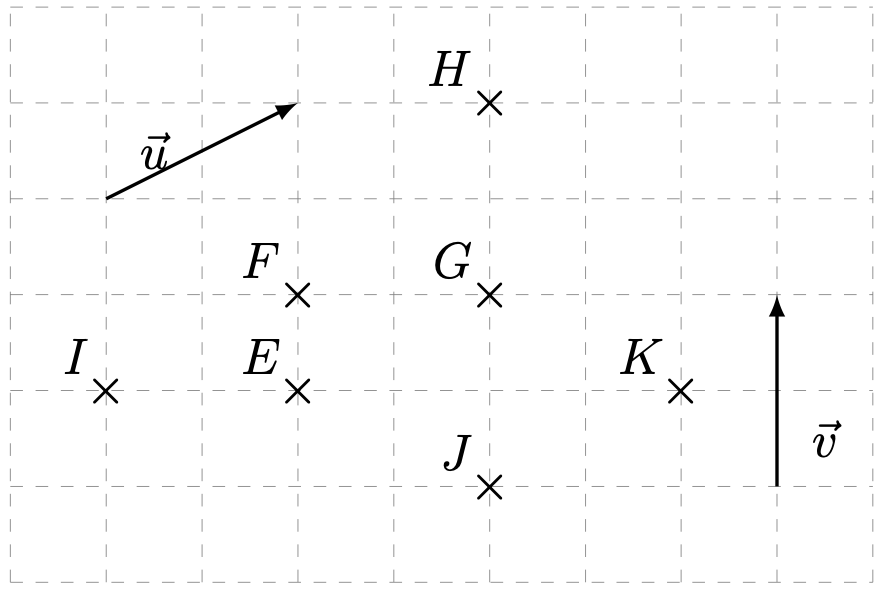
\includegraphics[width=6.5cm]{Images Exercice/Ex1-2-3}
\end{center}
\end{minipage}

\begin{Exercice} %4
\begin{minipage}{0.65\textwidth}

Sur la figure ci-contre, construire :
\begin{enumerate}
\item H, l'image de C par la translation de vecteur $ \overrightarrow{AB} $.
\item I, l'image de F par la translation de vecteur $ \overrightarrow{EG} $.
\item JKL, l'image du triangle DEG par la translation de vecteur $ \overrightarrow{BA} $.
\item M tel que C soit l'image de M par la translation de vecteur $ \overrightarrow{EB} $.
\end{enumerate}

\end{minipage} \hfill
\begin{minipage}{0.3\textwidth}
\begin{center}
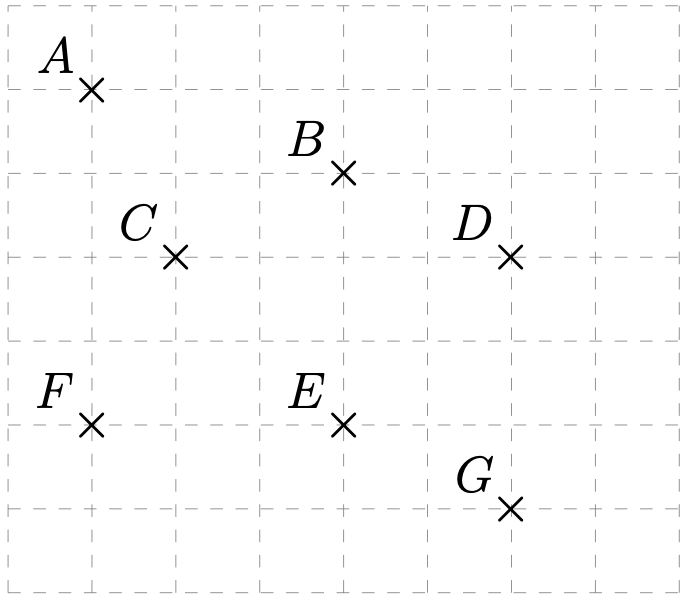
\includegraphics[width=4.5cm]{Images Exercice/Ex4}
\end{center}
\end{minipage} 

\end{Exercice}




\begin{Exercice} %5
\begin{minipage}{0.6\textwidth}

Sur la figure ci-contre, constituée de 6 carrés déterminer :
\begin{enumerate}
\item l'image de H par la translation de vecteur $ \overrightarrow{AE} $.
\item l'image de N par la translation de vecteur $ \overrightarrow{MB} $.
\item Trois vecteurs égaux à $ \overrightarrow{FD} $, différents de celui-ci.

\end{enumerate}

\end{minipage}
\begin{minipage}{0.35\textwidth}
\begin{center}

\includegraphics[width=3.8cm]{Images Exercice/Ex5}
\end{center}
\end{minipage}

\end{Exercice}




\begin{Exercice} %6

\begin{minipage}{0.65\textwidth}

Sur la figure ci-contre, constituée de 4 parallélogrammes, déterminer :
\begin{enumerate}
\item l'image de E par la translation de vecteur $ \overrightarrow{DH} $.
\item l'image de B par la translation de vecteur $ \overrightarrow{AG} $.
\item Trois vecteurs égaux à $ \overrightarrow{CE} $, différents de celui-ci.
\item un vecteur égal à $ \overrightarrow{IB} $, différents de celui-ci.
\end{enumerate}

\end{minipage}
\begin{minipage}{0.35\textwidth}
\begin{center}

\includegraphics[width=3.8cm]{Images Exercice/Ex6}
\end{center}
\end{minipage}

\end{Exercice}



\begin{Exercice} %7
\begin{minipage}{0.75\textwidth}

Sur la figure ci-contre, ABCD est un parallélogramme.
\begin{enumerate}
\item A quel autre vecteur est égal $ \overrightarrow{CD} $ ? $ \overrightarrow{CB} $ ? $ \overrightarrow{AD} $ ?.
\item Construire le point E tel que $ \overrightarrow{AE}=\overrightarrow{BA} $.
\item Construire le point F, image du point C par la translation de vecteur $ \overrightarrow{AD} $.
\end{enumerate}

\end{minipage} \hfill
\begin{minipage}{0.25\textwidth}
\begin{center}

\includegraphics[width=3.6cm]{Images Exercice/Ex7}
\end{center}
\end{minipage}

\end{Exercice}
\newpage


\begin{minipage}{\textwidth}
\begin{Exercice} %8
On considère six points A,B,C,D,E et F tels que ABCD et CDEF sont des parallélogrammes.
\begin{enumerate}
\item Faire une figure.
\item Écrire les égalités vectorielles correspondant à cette affirmation.
\item Montrer que ABFE est un parallélogramme.
\end{enumerate}
\end{Exercice} 
\end{minipage}
\vspace{0.5cm}


\begin{minipage}{\textwidth}
\begin{Exercice} %9
Soit ABC un triangle quelconque et I le milieu de [AB].
\begin{enumerate}
\item Faire une figure et construire le point I', image de I par la translation de vecteur $ \overrightarrow{BC} $.
\item Construire le point A', image de A par la translation de vecteur $ \overrightarrow{I'I} $.
\item Quelle est la nature du quadrilatère BCAA' ? Justifier.
\end{enumerate}
\end{Exercice} 
\end{minipage}
\vspace{0.5cm}

\subsection*{Somme de vecteurs}

\begin{Exercice} %10
\vspace{0.2cm}
\begin{minipage}{0.65\textwidth}

Sur la figure ci-contre, constituée de 6 carrés déterminer :
\begin{enumerate}
\item deux vecteur égaux à $\overrightarrow{HG}+\overrightarrow{GM}$.
\item deux vecteur égaux à $\overrightarrow{LK}+\overrightarrow{LF}$.
\item deux vecteur égaux à $\overrightarrow{AC}+\overrightarrow{GM}$
\item deux vecteur égaux à $\overrightarrow{AB}+\overrightarrow{DE}+\overrightarrow{HL}$
\end{enumerate}

\end{minipage}
\begin{minipage}{0.35\textwidth}
\begin{center}

\includegraphics[width=4cm]{Images Exercice/Ex10}
\end{center}
\end{minipage}

\end{Exercice}

\begin{Exercice} %11
\begin{minipage}{0.55\textwidth}
En utilisant la figure ci-contre, simplifier les égalités de vecteurs suivantes
\begin{enumerate}
\item $\overrightarrow{AE}+\overrightarrow{EO} = $
\item $\overrightarrow{AD}+\overrightarrow{AB} = $
\item $\overrightarrow{AO}+\overrightarrow{FC} = $
\item $\overrightarrow{BD}-\overrightarrow{BC} = $
\item $\overrightarrow{AE}+\overrightarrow{OF}+\overrightarrow{DO} = $
\item $\overrightarrow{OC}+\overrightarrow{BA}-\overrightarrow{OF} = $
\item $\overrightarrow{AB}+\overrightarrow{CD} = $
\item $\overrightarrow{AC}+\overrightarrow{OA}+\overrightarrow{FA} = $
\end{enumerate}

\end{minipage}
\begin{minipage}{0.45\textwidth}
\begin{center}

\includegraphics[width=6cm]{Images Exercice/Ex11}
\end{center}
\end{minipage}

\end{Exercice}


\begin{Exercice} %12
On considère un carré ABCD. Faire une figure puis...
\begin{enumerate}
\item Construire le point E tel que $ \overrightarrow{BE} = \overrightarrow{DC} + \overrightarrow{DB} $.
\item Construire le point F tel que $ \overrightarrow{CF} = \overrightarrow{AD} + \overrightarrow{BA} $.
\item Construire le point G tel que $ \overrightarrow{AG} = \overrightarrow{DA} + \overrightarrow{BC} $.
\end{enumerate}
\end{Exercice} 




\begin{Exercice} %13
Simplifier au maximum les sommes de vecteurs suivantes.
\begin{multicols}{3}
$\overrightarrow{AB}+\overrightarrow{BM} $\\

$\overrightarrow{AB}+\overrightarrow{BM}+\overrightarrow{MQ} $\\

$\overrightarrow{DC}+\overrightarrow{CD} $\\

$\overrightarrow{TD}+\overrightarrow{ST}+\overrightarrow{DA} $\\

$\overrightarrow{MP}+\overrightarrow{AM} $\\

$\overrightarrow{AB}+\overrightarrow{BC} +\overrightarrow{CA}$\\

\end{multicols}
\end{Exercice} 



\begin{Exercice} %14
Simplifier au maximum les sommes de vecteurs suivantes
\begin{multicols}{3}
$\overrightarrow{AB}-\overrightarrow{PB} $\\

$\overrightarrow{AB}+\overrightarrow{BM}-\overrightarrow{TM} $\\

$\overrightarrow{DC}-\overrightarrow{DC} $\\

$\overrightarrow{AC}-\overrightarrow{FC}+\overrightarrow{FT} $\\

$-\overrightarrow{SK}+\overrightarrow{MK} $\\

$\overrightarrow{AU}+\overrightarrow{BL} -\overrightarrow{BU}$\\

\end{multicols}
\end{Exercice} 



\begin{Exercice} %15
Le but de l'exercice est de démontrer la règle du parallélogramme : Soit A, B, C et D quatre points du plan. ABCD est un parallélogramme si et seulement si $\overrightarrow{AB}+\overrightarrow{AD} =\overrightarrow{AC}$
\begin{enumerate}
\item On suppose que ABCD est un parallélogramme.
\begin{enumerate}
\item A quel vecteur est égal le vecteur $ \overrightarrow{AB} $ ?
\item Ajouter $ \overrightarrow{AD} $ à chaque membre de l'égalité de la question précédente. Qu'obtient-on ?
\end{enumerate}
\item On suppose désormais que $\overrightarrow{AB}+\overrightarrow{AD} =\overrightarrow{AC}$.
\begin{enumerate}
\item Décomposer le vecteur $ \overrightarrow{AC} $ selon D grâce à la relation de Chasles.
\item En déduire que $ \overrightarrow{AB}=\overrightarrow{DC} $ et conclure.
\end{enumerate}
\end{enumerate}
\end{Exercice} 



\begin{Exercice} %16
On considère un parallélogramme RSTU de centre O. On place les points M et N sur le
segment [RS] et [UT] tels que $ \overrightarrow{MS}=\overrightarrow{UN} $.\\
 Montrer que O est le milieu de [MN] : (Ne pas hésiter à faire une figure pour visualiser le problème).
\end{Exercice} 

\newpage

\subsection*{Produit d'un vecteur par un réel}

\begin{Exercice} %17
Des points ont été placés sur une droite ci-dessous. La distance entre deux points consécutifs est toujours la même.\\
\begin{center}
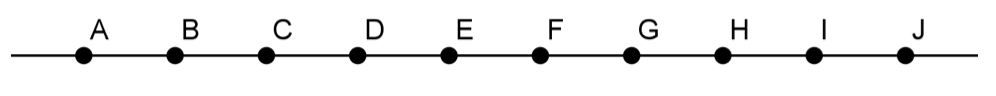
\includegraphics[scale=0.9]{Images Exercice/Ex17}
\end{center}
\begin{enumerate}
\item Compléter les égalités suivantes avec des réels.
\begin{multicols}{3}
\begin{minipage}{0.3\textwidth}
$ \overrightarrow{AE}= ... \overrightarrow{AB} $\\
$ \overrightarrow{BG}= ... \overrightarrow{IF} $\\
\end{minipage}
\begin{minipage}{0.3\textwidth}
$ \overrightarrow{DF}= ... \overrightarrow{IH} $\\
$ \overrightarrow{BH}= ... \overrightarrow{CE} $\\
\end{minipage}
\begin{minipage}{0.3\textwidth}
$ \overrightarrow{HJ}= ... \overrightarrow{CI} $\\
$ \overrightarrow{JA}= ... \overrightarrow{BF} $
\end{minipage}
\end{multicols}
\item Déterminer un vecteur égal aux vecteurs suivants :
\begin{multicols}{3}
\begin{minipage}{0.3\textwidth}
$ 2\overrightarrow{DE}=  $\\
$ -2\overrightarrow{CE}=  $\\
\end{minipage}
\begin{minipage}{0.3\textwidth}
$ 3\overrightarrow{FI}=  $\\
$ -\dfrac{3}{2}\overrightarrow{FD}=  $\\
\end{minipage}
\begin{minipage}{0.3\textwidth}
$ \dfrac{3}{2}\overrightarrow{BH}= $\\
$ -\dfrac{2}{5}\overrightarrow{AF}= $\\
\end{minipage}
\end{multicols}
\end{enumerate}

\end{Exercice} 

\begin{Exercice} %18
Sur la figure ci-dessous, construire les points H, I, J, K, L, M,N définis par les relations vectorielles suivantes.
\begin{minipage}{0.45\textwidth}
\vspace{0.3cm}
\begin{enumerate}
\item $\overrightarrow{EH}=2\overrightarrow{u}$
\item $\overrightarrow{EI}=-\dfrac{1}{2}\overrightarrow{u}$
\item $\overrightarrow{FJ}=3\overrightarrow{v}$
\item $\overrightarrow{FK}=2\overrightarrow{w}$
\item $\overrightarrow{GL}=\overrightarrow{w}+2\overrightarrow{u}$
\item $\overrightarrow{GM}=-5\overrightarrow{w}$
\item $\overrightarrow{NE}=\overrightarrow{v}-\overrightarrow{w}-2\overrightarrow{u}$
\end{enumerate}

\end{minipage}
\begin{minipage}{0.5\textwidth}
\begin{center}
\begin{center}
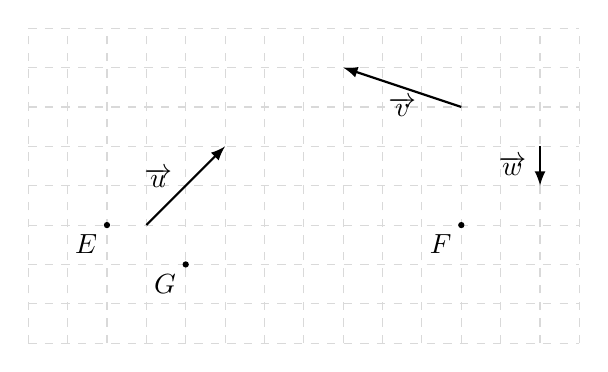
\begin{tikzpicture}[x=0.5cm,y=0.5cm]
% Définition des limites
\def\xmin{-2}
\def\xmax{12}
\def\ymin{-1}
\def\ymax{7}

% Grille avec step=1 pour correspondre aux coordonnées
\draw[gray!30, dashed] (\xmin,\ymin) grid[step=1] (\xmax,\ymax);

% Points
\fill (0,2) circle (0.08) node[below left] {$E$};
\fill (2,1) circle (0.08) node[below left] {$G$};
\fill (9,2) circle (0.08) node[below left] {$F$};

% Vecteur u (de E vers le haut à droite)
\draw[->,>=latex,thick] (1,2) -- (3,4);
\draw (1.3,3.2) node {$\overrightarrow{u}$};

% Vecteur v (horizontal vers la droite)
\draw[->,>=latex,thick] (9,5) -- (6,6);
\draw (7.5,5) node {$\overrightarrow{v}$};

% Vecteur w (vertical vers le bas)
\draw[->,>=latex,thick] (11,4) -- (11,3);
\draw (10.3,3.5) node {$\overrightarrow{w}$};

\end{tikzpicture}
\end{center}
\end{center}
\end{minipage}

\end{Exercice}




\begin{Exercice} %19
Simplifier au maximum les sommes de vecteurs suivantes
\begin{multicols}{3}
\begin{itemize}[label=\textcolor{Couleur6}{$\bullet$}]
\item $3\overrightarrow{u}+2\overrightarrow{u}+4\overrightarrow{u} $\\

\item $2\overrightarrow{u}-(3\overrightarrow{u}+4\overrightarrow{u}) $\\

\item $3\overrightarrow{u}-2\overrightarrow{u}+\overrightarrow{u} $\\

\item $5\overrightarrow{u}-2\overrightarrow{u}+\overrightarrow{u} $\\

\item $\overrightarrow{u}+2(\overrightarrow{u}+5\overrightarrow{u}) $\\

\item $\dfrac{3}{7}\overrightarrow{u}+\dfrac{6}{7}\overrightarrow{u}+\dfrac{5}{7}\overrightarrow{u} $\\

\item $-7\overrightarrow{u}+\overrightarrow{u}+8\overrightarrow{u} $\\

\item $\dfrac{2}{5}\overrightarrow{u}-\dfrac{4}{5}\overrightarrow{u}+\dfrac{1}{10}\overrightarrow{u} $\\

\item $3(\overrightarrow{u}-2\overrightarrow{u})+2(3\overrightarrow{u}+4\overrightarrow{u}) $\\
\end{itemize}
\end{multicols}
\end{Exercice} 

\newpage

\begin{Exercice} %20
En utilisant la relation de Chasles, simplifier les expressions vectorielles suivantes.
\begin{multicols}{3}
$2\overrightarrow{AB}+2\overrightarrow{BC}$\\
$4\overrightarrow{AB}+2\overrightarrow{BA}$\\
$2\overrightarrow{AB}+\overrightarrow{BC}+\overrightarrow{CA}$
\end{multicols}
\end{Exercice} 



\begin{Exercice} %21
Soient A, B, C, D et E cinq points du plan et M le point tel quel\\
\begin{center}
$\overrightarrow{AM}=\dfrac{1}{4}\overrightarrow{AE}+\dfrac{1}{4}\overrightarrow{CB}-\dfrac{1}{4}\overrightarrow{DC}+\dfrac{1}{4}\overrightarrow{AC}-\dfrac{1}{4}\overrightarrow{CE}+\dfrac{1}{4}\overrightarrow{DB}$
\end{center}
Montrer que M est le milieu de [AB].

\end{Exercice}


\begin{Exercice} %22
Le but de l'exercice est de montrer que dans tout quadrilatère, les milieux des côtés forment un parallélogramme. Ce résultat est connu sous le nom de théorème de Varignon. On considère donc ABCD un quadrilatère quelconque, ainsi que I, J, K et L, milieux respectifs de [AB], [BC], [CD] et [DA].
\begin{enumerate}
\item Décomposer le vecteur $ \overrightarrow{AC} $ selon B grâce à la relation de Chasles.
\item On rappelle que I et J sont les milieux de [AB] et [BC]. Quelles égalités vectorielles peut-on écrire ?
\item Montrer alors que $ \overrightarrow{AC}=2\overrightarrow{IJ} $.
\item Montrer de même que $ \overrightarrow{AC}=2\overrightarrow{LK} $ et conclure.
\end{enumerate}
\end{Exercice}


}
